\documentclass[10pt]{article}

\usepackage{lipsum}
\usepackage{url}
\usepackage{float}
\usepackage{amsmath}
\usepackage{enumitem}
\usepackage{graphicx}
\usepackage{caption}
\usepackage{subcaption}
\usepackage{rotating}
\usepackage{geometry}
\usepackage{listings}
\usepackage{hyperref}
\usepackage[T1]{fontenc}
\usepackage[numbered]{matlab-prettifier}

\newcommand{\documentTitle}{Lab 5 - Signal Analysis and Characterization}
\newcommand{\documentAuthor}{Andrew Pham, Aneel Damaraju}
\newcommand{\courseTitle}{ELEC 240}
\newcommand{\testDate}{October 2, 2018}
\newcommand{\reportDate}{October 16, 2018}

\geometry{margin=1in}
\lstset{
    tabsize=4,
    basicstyle={\ttfamily},
    captionpos=b,
    belowskip=1em,
    aboveskip=1em,
    numbers=left,
	escapechar=\@,
}

\title{
    \textbf{\courseTitle} \\
    \textbf{\documentTitle} \\
    \bigskip
    \textbf{\large{Test performed: \testDate}} \\
    \textbf{\large{Report submitted: \reportDate}} \\
    \bigskip
    \bigskip
}
\author{\documentAuthor}
\date{}

\begin{document}

\maketitle

\newpage

\section{Objective}

The first objective of this lab was to learn how to generate a virtual signal with LabView and vary the signal's parameters. The second objective of the lab was to learn how to acquire a signal in LabView from an external source like our VirtualBench function generator and then perform frequency analysis on the acquired signal. The third and final objective of the lab was to modify the circuit from Lab 4 so that we could perform speech analysis as well as analyze an unknown signal. 

\medskip

%\textit{Note (To be deleted): Think of this test report as a document with your peers as your readers. This means you can assume a similar knowledge background as you. Your readers should be able to easily understand what is going on, and also be able to repeat your lab results based on your document and all references you cite.}

%\textit{For the Objective section, identify the test you performed and its objectives. The objectives of the test are important to state because they are usually analyzed in the conclusion to determine whether the test succeeded.}

\section{Materials}

\begin{itemize}
	\item Virtual Bench (Software, Oscilloscope, Function Generator, DC Power Supply)
	\item LabView
	\item BNC Male to Clips cord
	\item BNC T connector
	\item Oscilloscope Probe
	\item Breadboard (with setup from Lab 4
	\item 2 10 cm length wires (with 6 mm stripped on each end)
	\item Digital Multimeter
	\item 2.2 $k\Omega$ resistor
	\item 033 $\mu F$ capacitor
	\item Telephone handset
	\item Dynamic microphone
	\item Smartphone (or some device to play audio from a speaker)
	
\end{itemize}

\medskip

%\textit{Note (To be deleted): Provide a bullet point list of components, software tools, and hardware (such as the NI VirtualBench or DMM) used during the lab}

\section{Test Description}

In Experiment 5.1, Part A, we focused on generating a signal in Labview by configuring circuit components on the block diagram pane in Labview. Once we created a configuration to generate a circuit, we created a spectrum analyzer in Part B by adding a Fast Fourier Transformer to the configuration and observed how varying the parameters of both the signal and measurement tools could affect the power spectrum graph. 

In Experiment 5.2, Part A, we acquired a signal from the NI VirtualBench by connecting the Data Acquisition Card (DAQ) within the PC running the LabView software via a DAQ cable. In this step, we also had to modify the previous configuration from Experiment 5.1 so that the circuit would accept an external signal. We achieved this by adding a DAQ assistant block so that LabView would read the incoming signal from the DAQ cable. In Part B, we explored the spectrum of triangle waves and how it varied as we tweaked the symmetry of the triangle wave. We also explored the spectrum of square waves and how it varied as we tweaked the duty cycle of the square wave. In Part C, we observed the spectrum and frequency response of a low-pass RC circuit by testing the circuit response at various frequencies. 

In Experiment 5.3, Part A, we explored the spectrum of speech signals by observing the spectral graph generated by making various vowel sounds and whistling with our mouths. By observing the spectra of these various signals, we estimated the approximate bandwidth for speech. In Part B, we modified the sound circuit from Lab 4 to spectrally analyze the Mystery Signal to determine how it achieves the effect of sounding like it was always ascending. 

\medskip

%\textit{Note (To be deleted): This section provides a summary of the test your team performed. Give enough information so readers can understand what you did, but do not go into the details of every step.}

\subsection{Pre-Lab Calculations and Schematics}

No pre-lab calculations were necessary; however, we needed an understanding of decibels and their relation to power in order to perform the experiments in the lab. The standard definition of power ration in decibels is as follows:

$$ \text{power ratio in decibels} = 10log(\frac{P_1}{P_0})$$

Since power across a load resistor can be defined as $$P = V^2/R$$then we can re-express the power ratio equation in a more convenient form as follows: $$\text{power ratio in decibels} = 10log(\frac{V_1^2/R_L}{V_0^2/R_L}) = 20log(\frac{V_1}{V_0})$$

With this expression of a power ratio, we can more conveniently express the ratio of sound pressure levels as $$\text{SPL} = 20log(\frac{p}{p_0})$$ where $p_0$ is the reference sound pressure 

\medskip

%\textit{Note (To be deleted): Include the homework pre-calculations and schematics that serve as the initial setup for the test. Briefly explain the importance of each item you include. You may want to number your equations/figures so you can refer to them in later sections. Including photos of handwritten work is okay.}

\section{Results and Discussion}

\subsection{Experiment 5.1: Virtual Instruments with Labview }
\qquad We begin by working in Labview, and generating a simple signal. First, a dial, numeric value and waveform graph were added to the front panel of the project. Then on the block diagram, a sine waveform was connected to the dial and connected to the numeric value and a white noise generator and the sine wave output were added and output to the graph. The block diagram was also wired so that the dial controls sine frequency and the value controls the amplitude. 

For Part B, we created a spectrum analyzer, to hopefully decode our noisy sine wave that is seen on the waveform graph. This is pretty straightforward thanks to Labview, and can be done simply by adding a power spectrum and power spectrum graph, and then assigning the entire graph to a while loop that continuously refreshes the power spectrum displayed. With the frequency spectrum set to 200Hz, a screenshot can be seen below in Fig \ref{fig:200hznoisy}

\begin{centering}
	\begin{figure} [H]
		\centering
		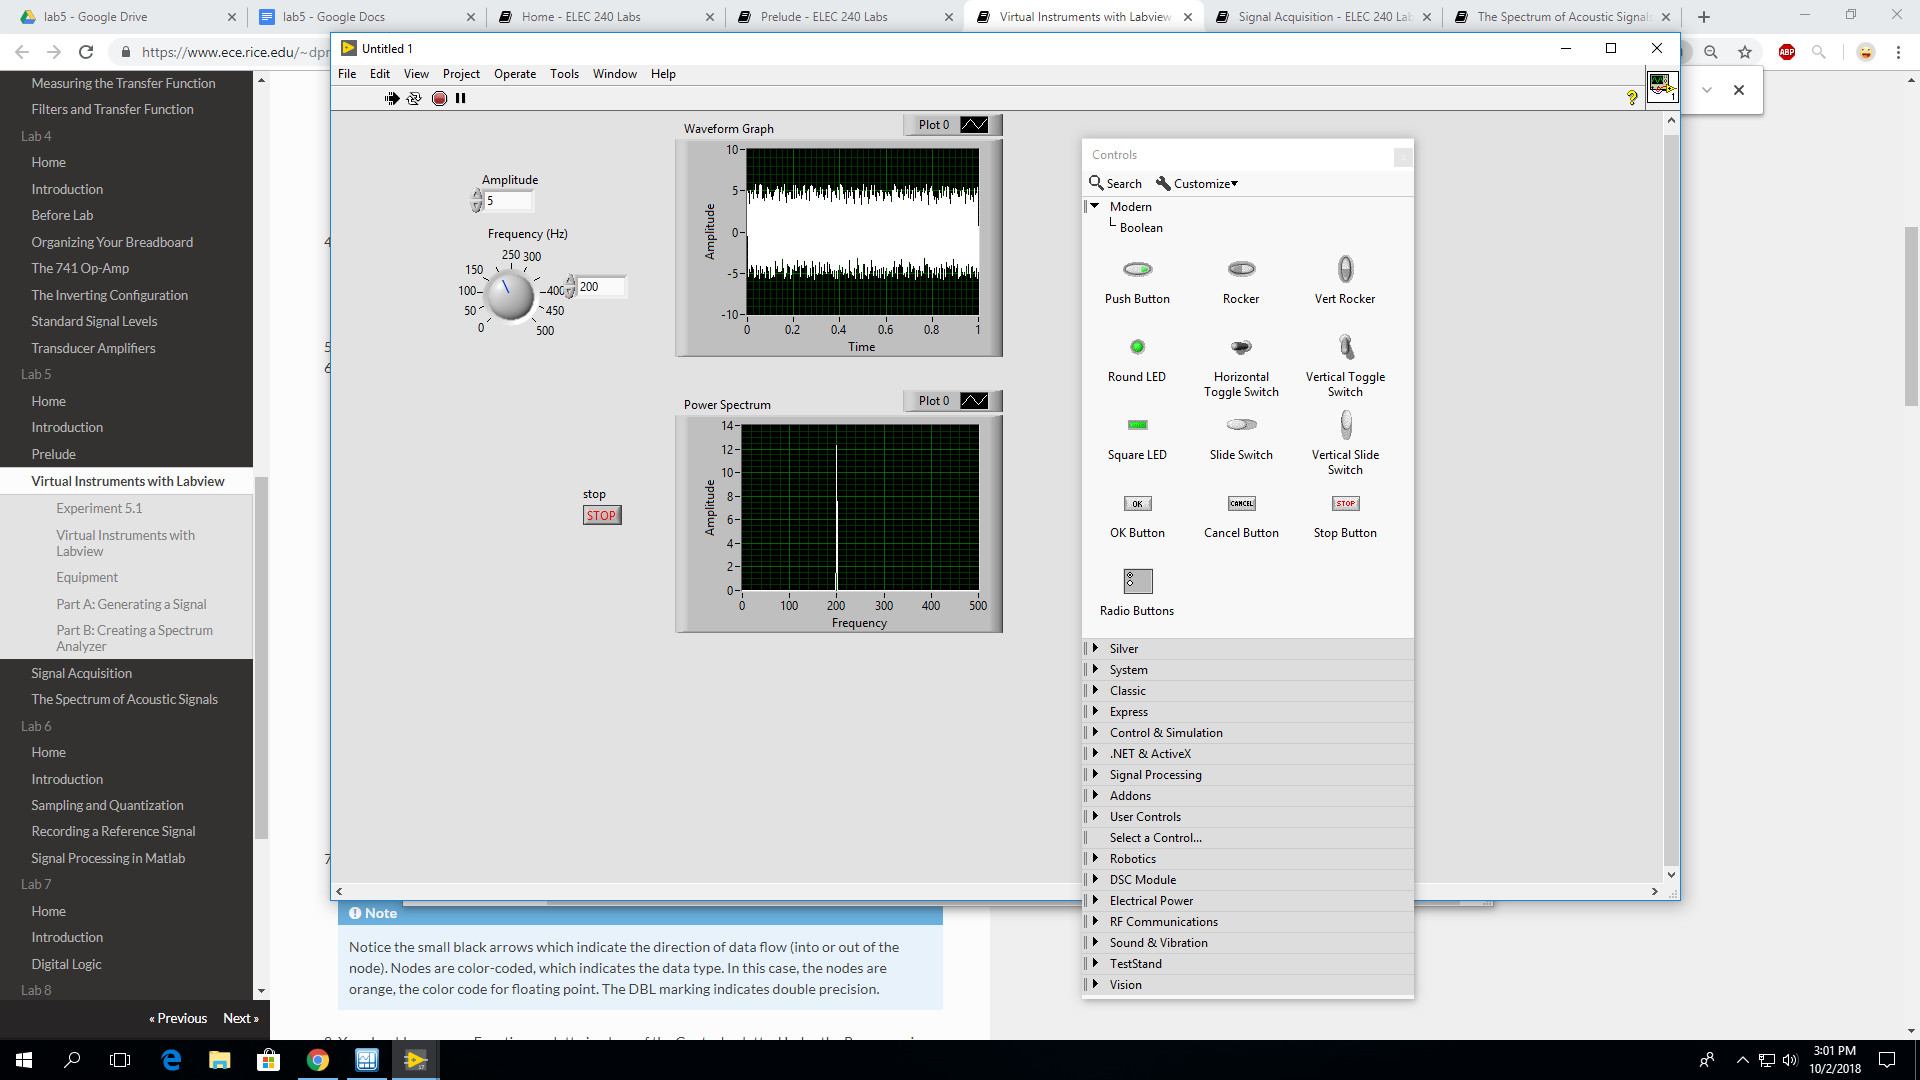
\includegraphics[scale=0.22]{images/200hzbasicspectralplot.png}\
		\caption{Spectral Plot of 200 Hz Noisy Sine Wave}
		\label{fig:200hznoisy}
	\end{figure}
\end{centering}

Through changing the frequency the output of the power spectrum would shift, but the high amplitude of the noise, along with its pseudo random nature made it difficult to find any discernible patterns in the spectra.

Through changing the controls, there were a few changes noticed in the in the output. The Db switch causes the offet values of the output to go to zero, while rescaling to magnifying the peaks. There were two different averaging modes that seemed to make the most impact, peak hold, which would record and hold peaks through frequency changes, and RMS averaging, which was useful to reduce the white noise effect. Finally, there was the weighting mode, linear simply holds the frequency and exponential causes smoothing due to the nature of exponential averaging.

The block diagram used to generate the circuit can be observed below in Fig \ref{fig:51block}
\begin{centering}
	\begin{figure} [H]
		\centering
		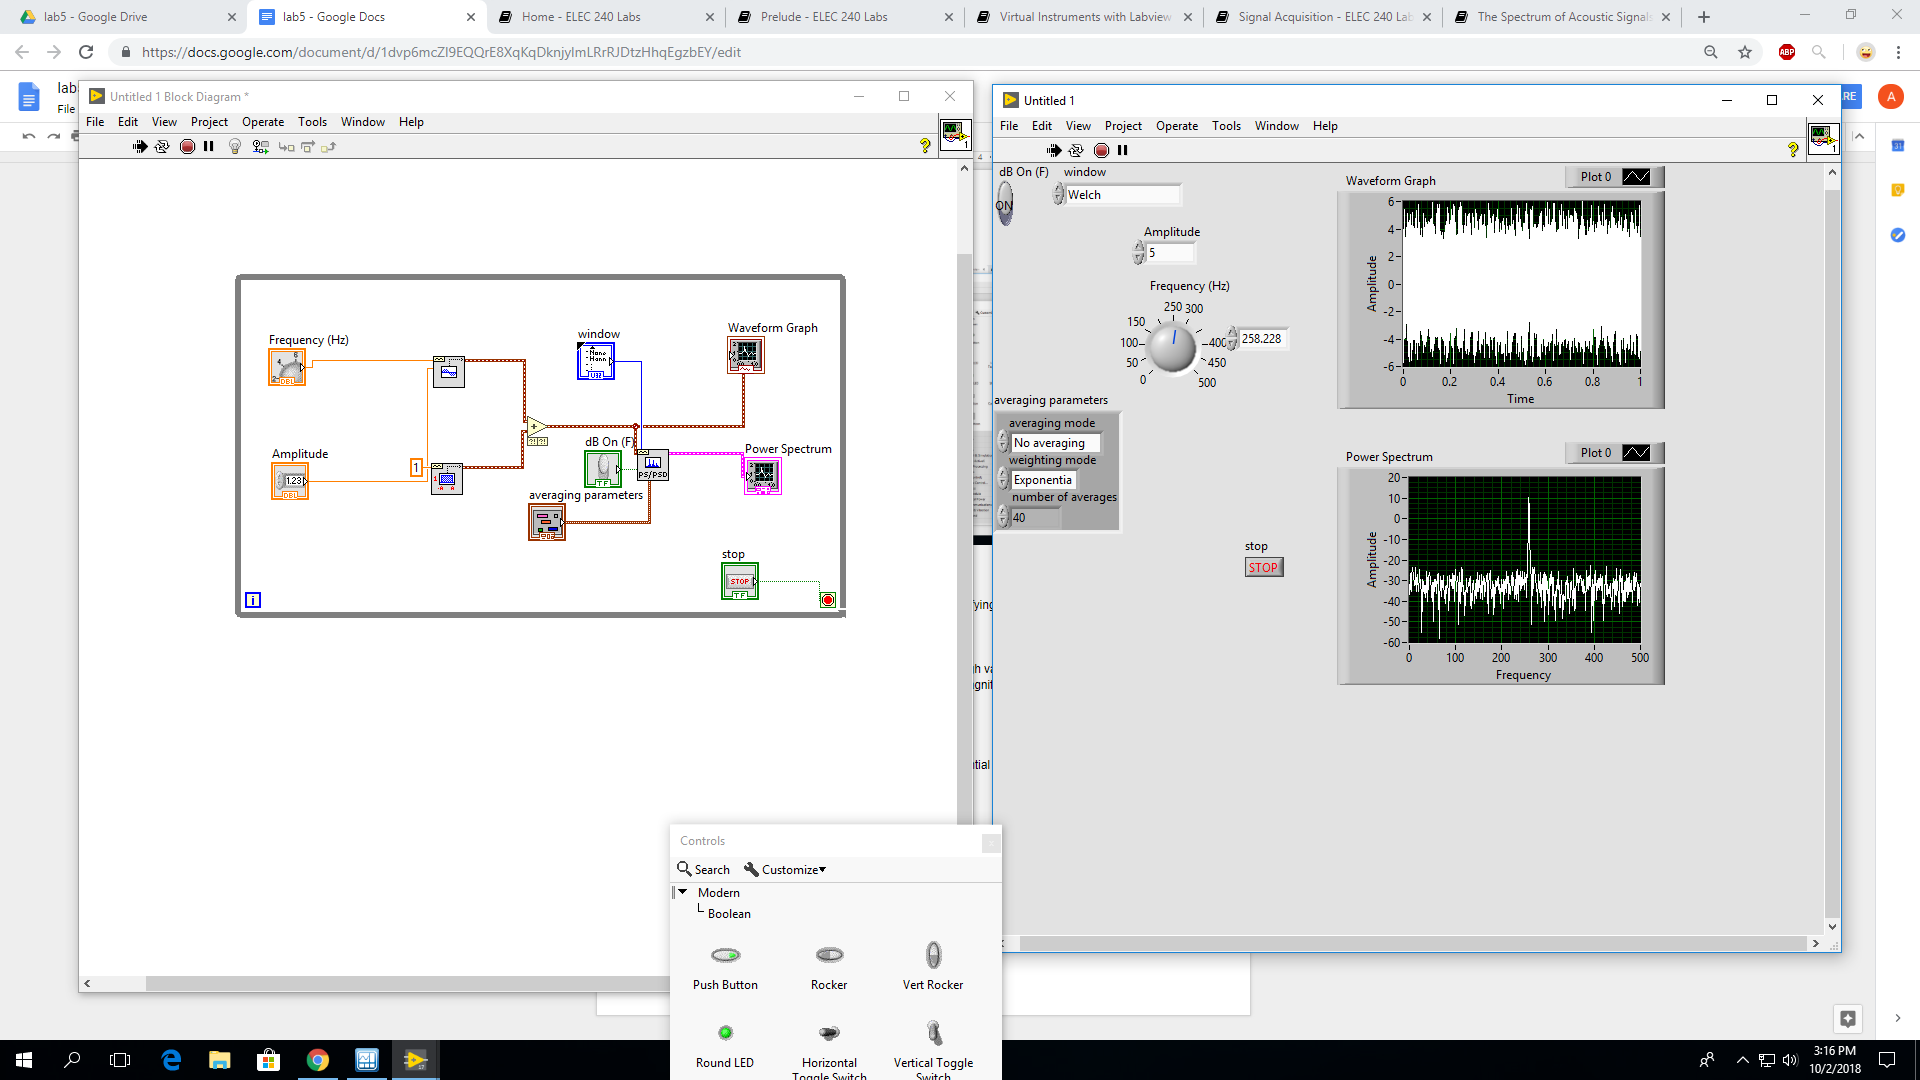
\includegraphics[scale=0.22]{images/51blockdiagram.png}\
		\caption{Block Diagram of Noisy Sine Wave Circuit}
		\label{fig:51block}
	\end{figure}
\end{centering}

\subsection{Experiment 5.2: Signal Acquisition}

As the name of the section implies, this section uses a DAQ cable for signal acquisition. The setup for this requires use of the Labview DAQ assistance, and controlling the number of samples and the rate of the DAQ. As seen below in Fig \ref{fig:52block}, the VI is ready to acquire signals.

\begin{centering}
	\begin{figure} [H]
		\centering
		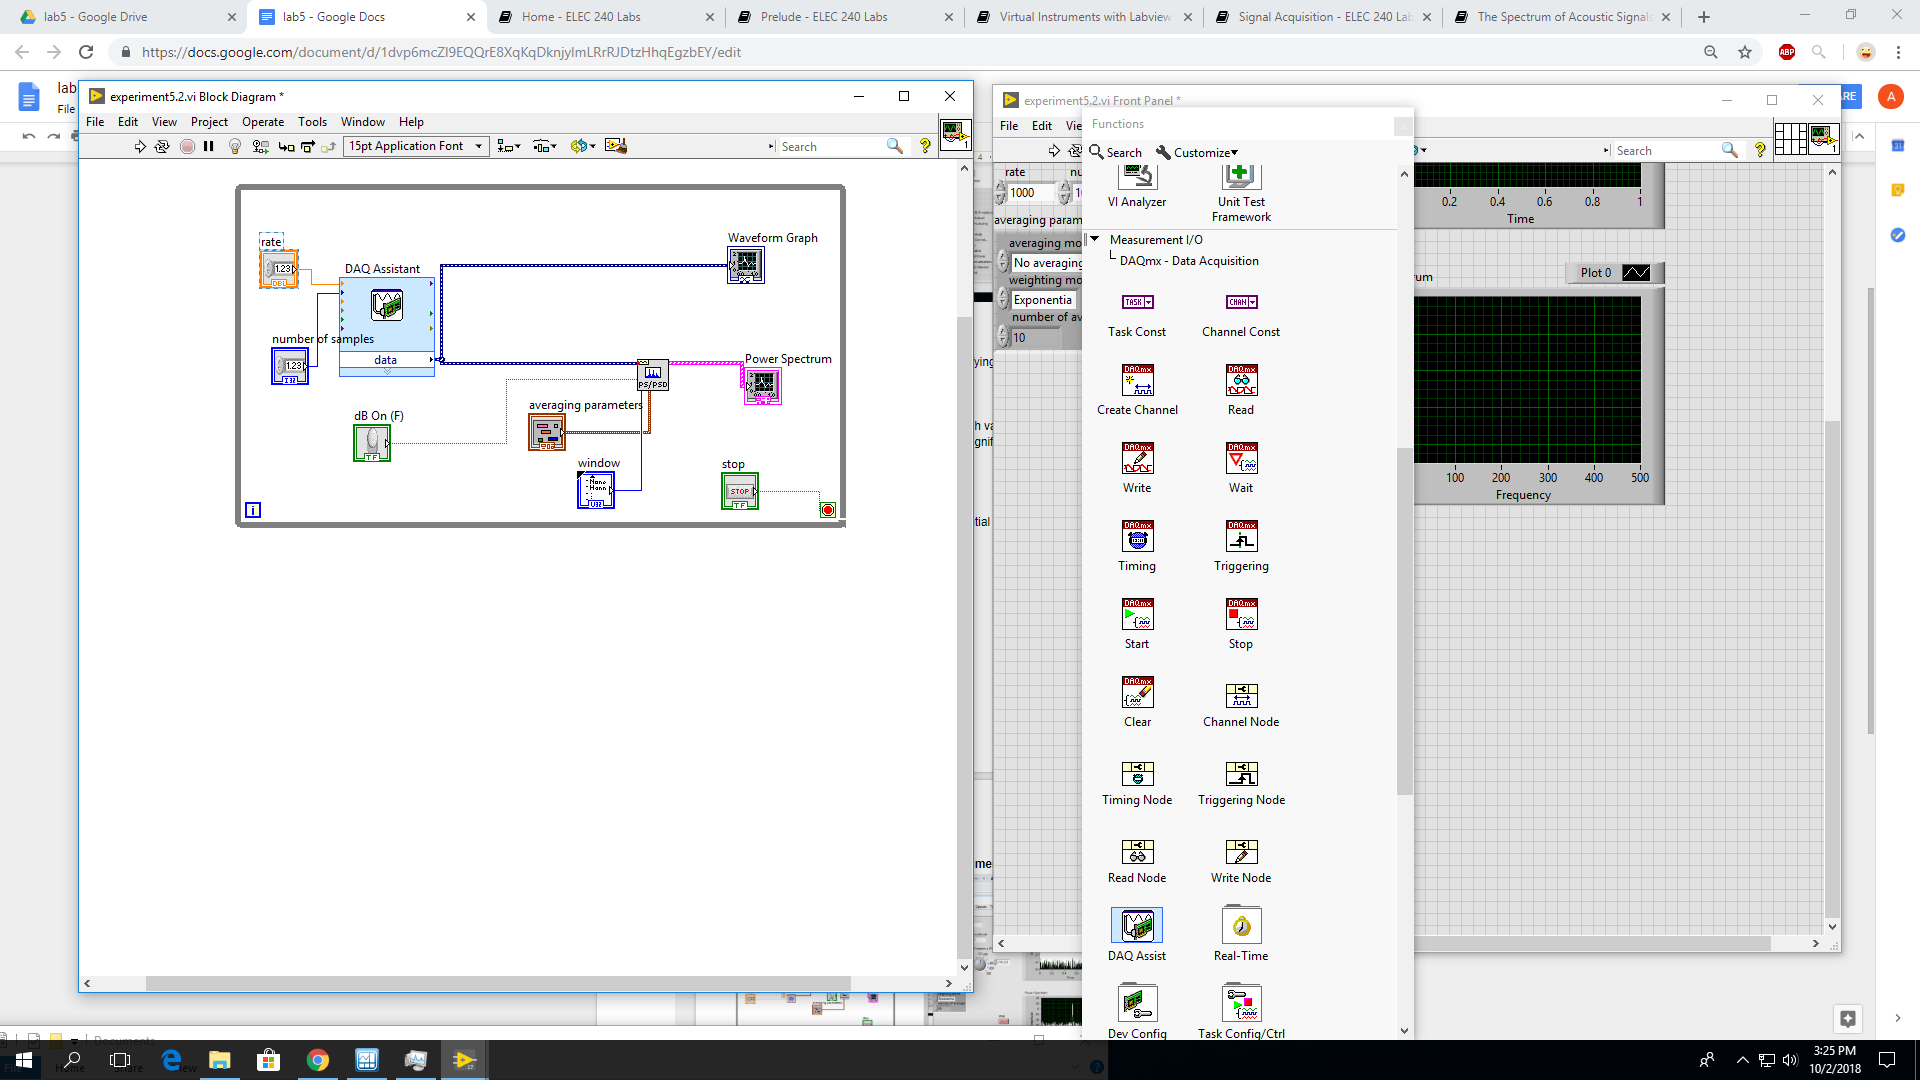
\includegraphics[scale=0.22]{images/52modifiedblock.png}\
		\caption{Block Diagram for Signal Acquisition Circuit}
		\label{fig:52block}
	\end{figure}
\end{centering}

Once it is clear that the VI is functioning, scaling the x and y on the output graph to a reasonable scale is next, as seen in Fig \ref{fig:2vpp500hz}. 

\begin{centering}
	\begin{figure} [H]
		\centering
		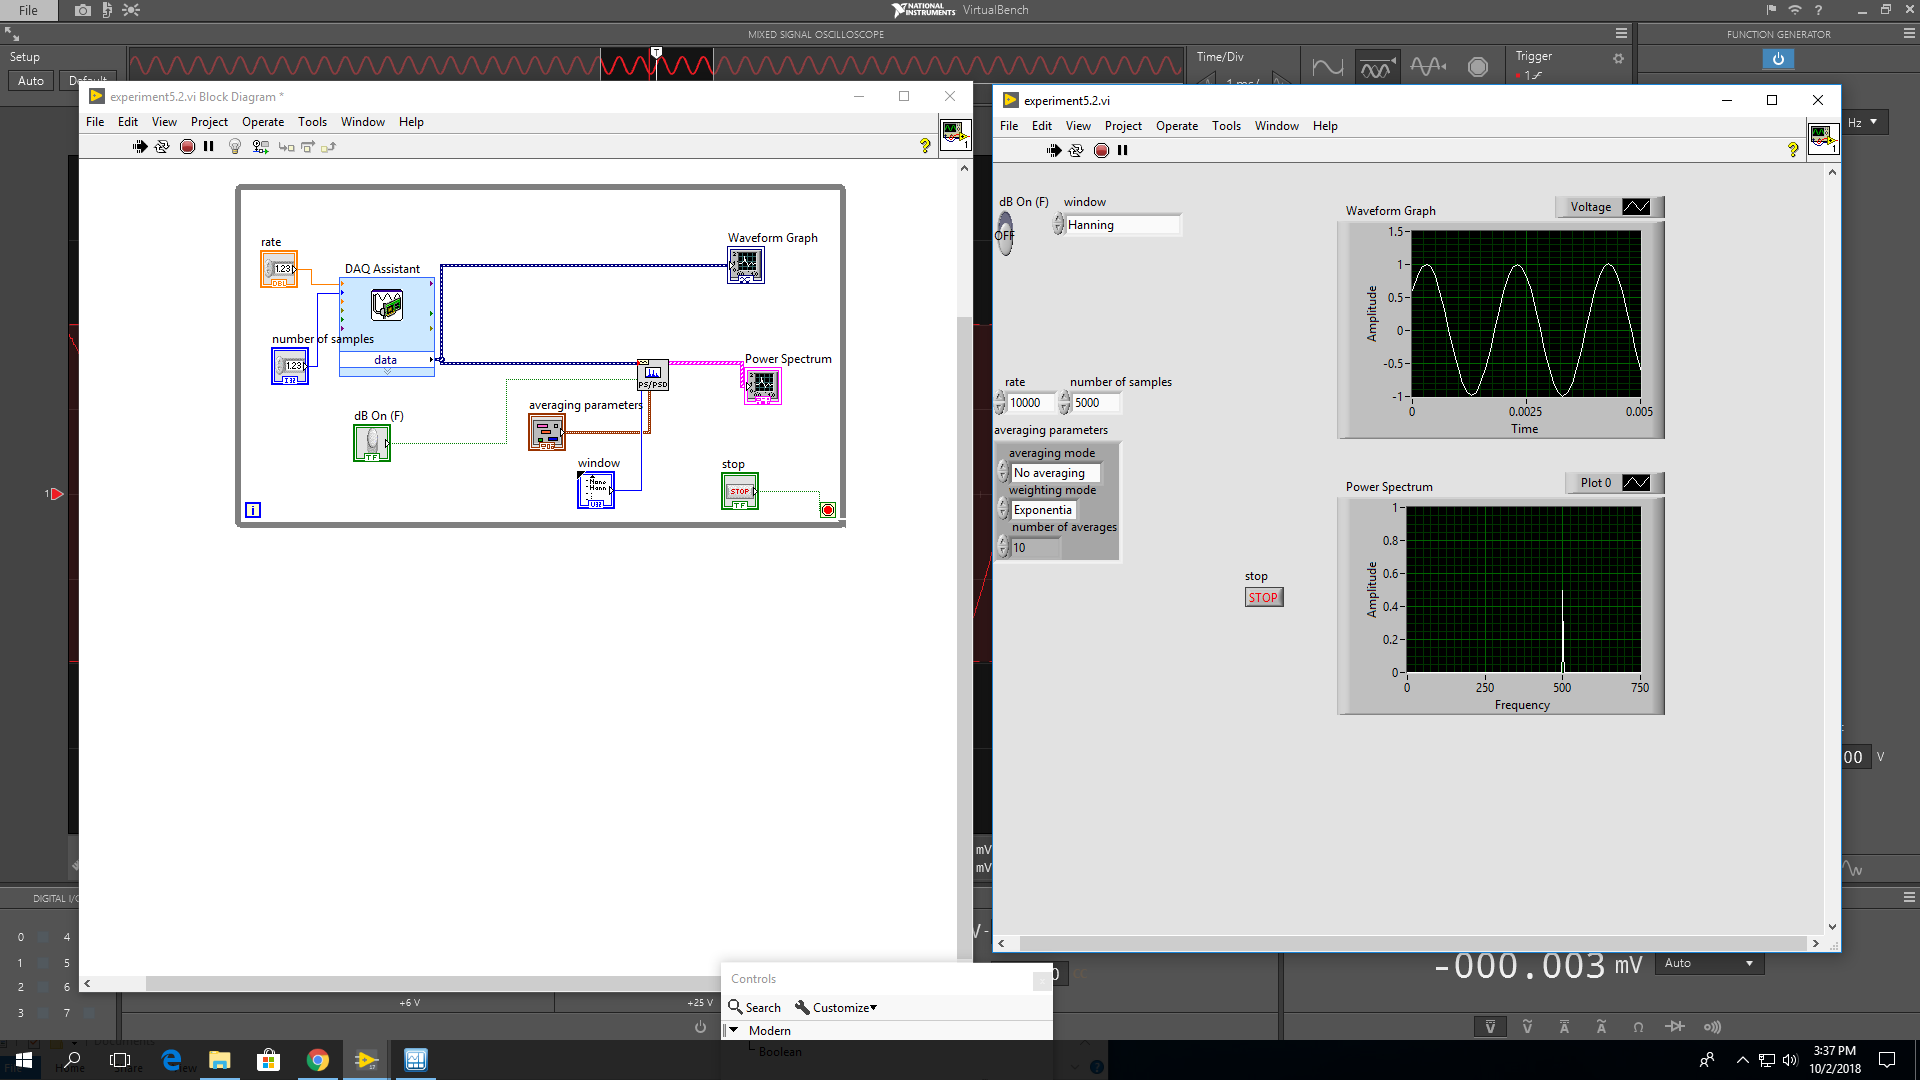
\includegraphics[scale=0.22]{images/2vpp500hz.png}
		\caption{Power Spectrum of 2 $V_{pp}$, 500 hz Sinusoid}
		\label{fig:2vpp500hz}
	\end{figure}
\end{centering}

By adding other tool blocks to measure the amplitude and the RMS Voltage, we found that the amplitude and RMS Voltage to be amplitude = 670 mV, rms = 0.25 V, as seen below in Fig \ref{fig:2vpp500hzextra}

\begin{centering}
	\begin{figure} [H]
		\centering
		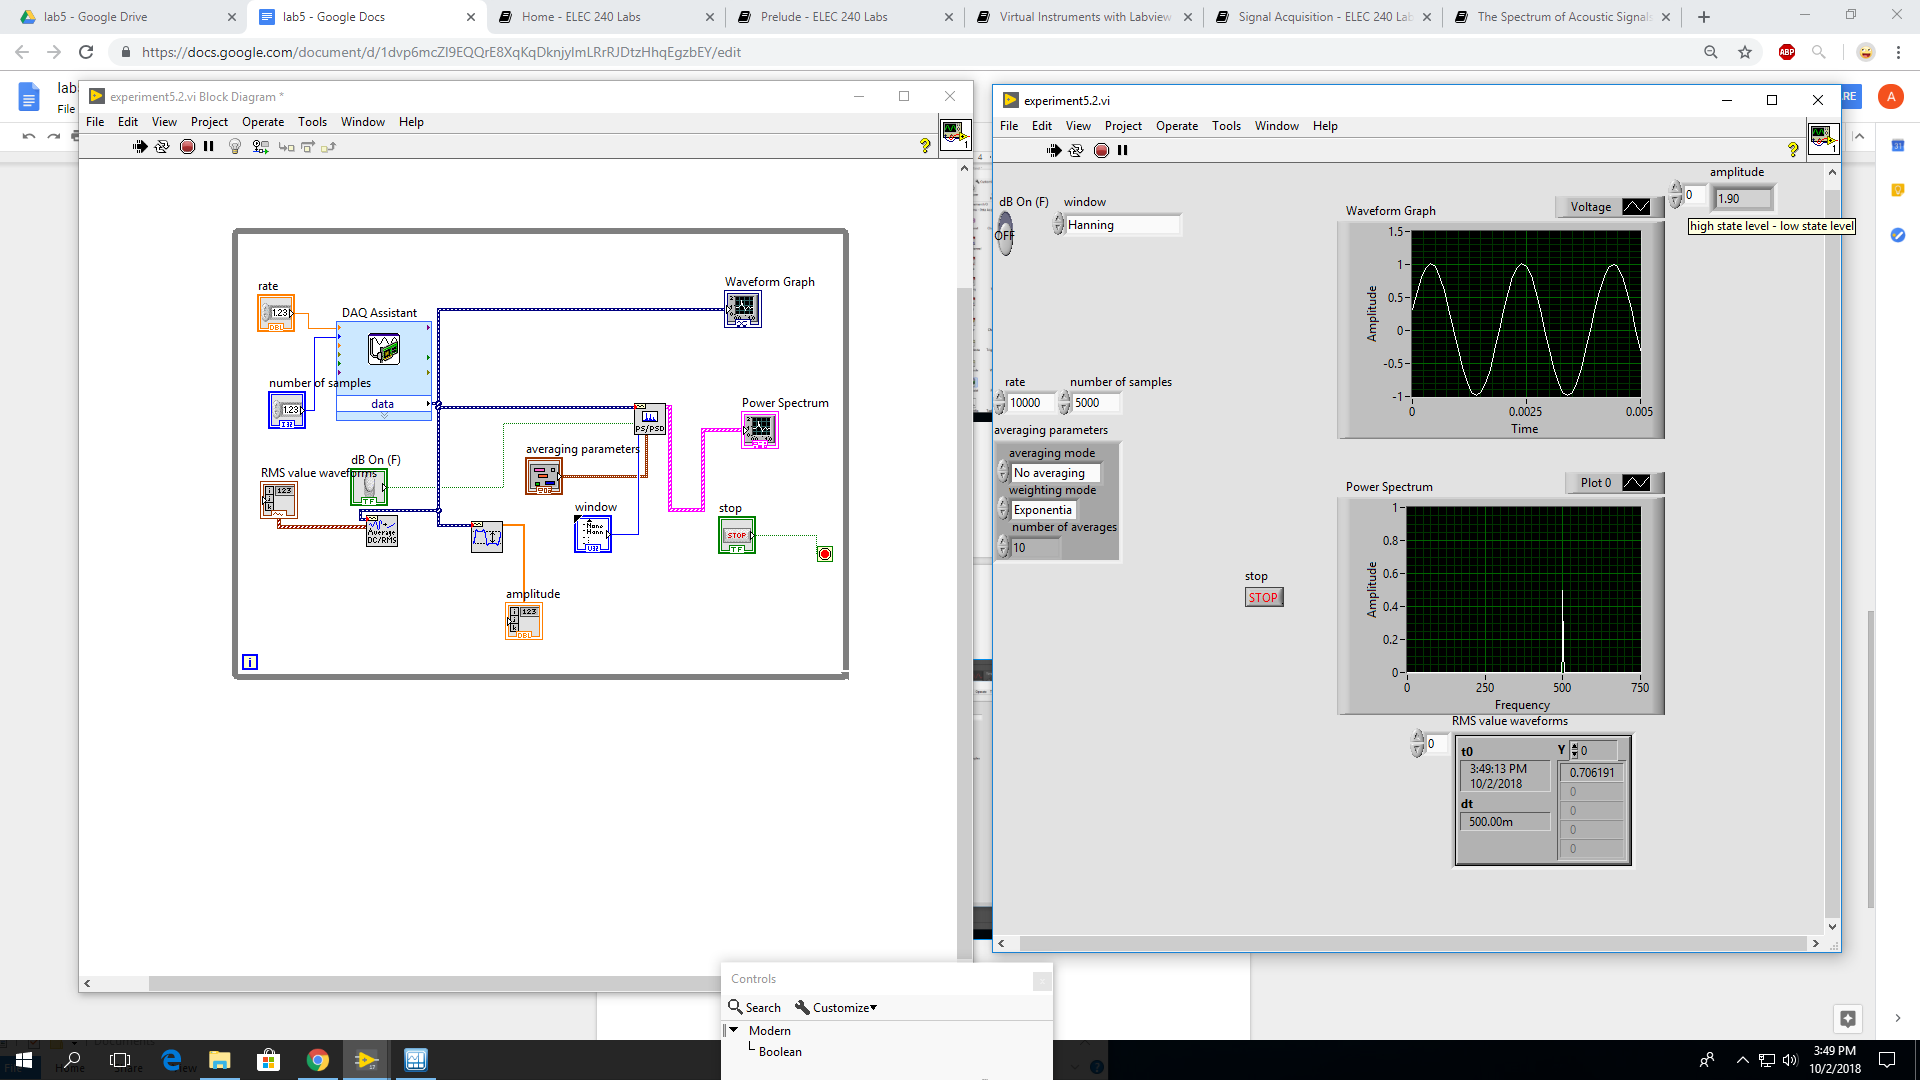
\includegraphics[scale=0.22]{images/2vpp500hzwithrmsandamplitude.png}
		\caption{Power Spectrum of 2 $V_{pp}$, 500 hz Sinusoid with Amplitude and RMS measurements}
		\label{fig:2vpp500hzextra}
	\end{figure}
\end{centering}


With the FGen disconnected, the input only receives noise being picked up from the external environment.

In Part B, we varied the symmetry of the input slants and observed output waveform. Inputting a square wave leads to evenly spaced spikes with exponentially decaying amplitude, increasing the duty cycle over 50 leads to an increase in spectral spikes, implying that the new waveform is described by more sine waves than before. Changing to a log-y scale, the harmonics do fall off in a hyperbolic fashion. With the log log plot, the 1/f fall of does obey a linear 20dB/ decade slope. For a triangle wave, the slope is now 40 dB/ decade as expected. for a 15\% square wave, the signal acts like a pulse and obeys the sinc function falloff. 

In Part C, we wired the circuit to an RC lowpass (reading the voltage across the resistor). With the function generator acting as $V_in$ with a 50 Hz sine wave, it is clear that halving the frequency drops the output by around 6 dB as seen in Fig \ref{fig:124}

\begin{centering}
	\begin{figure} [H]
		\centering
		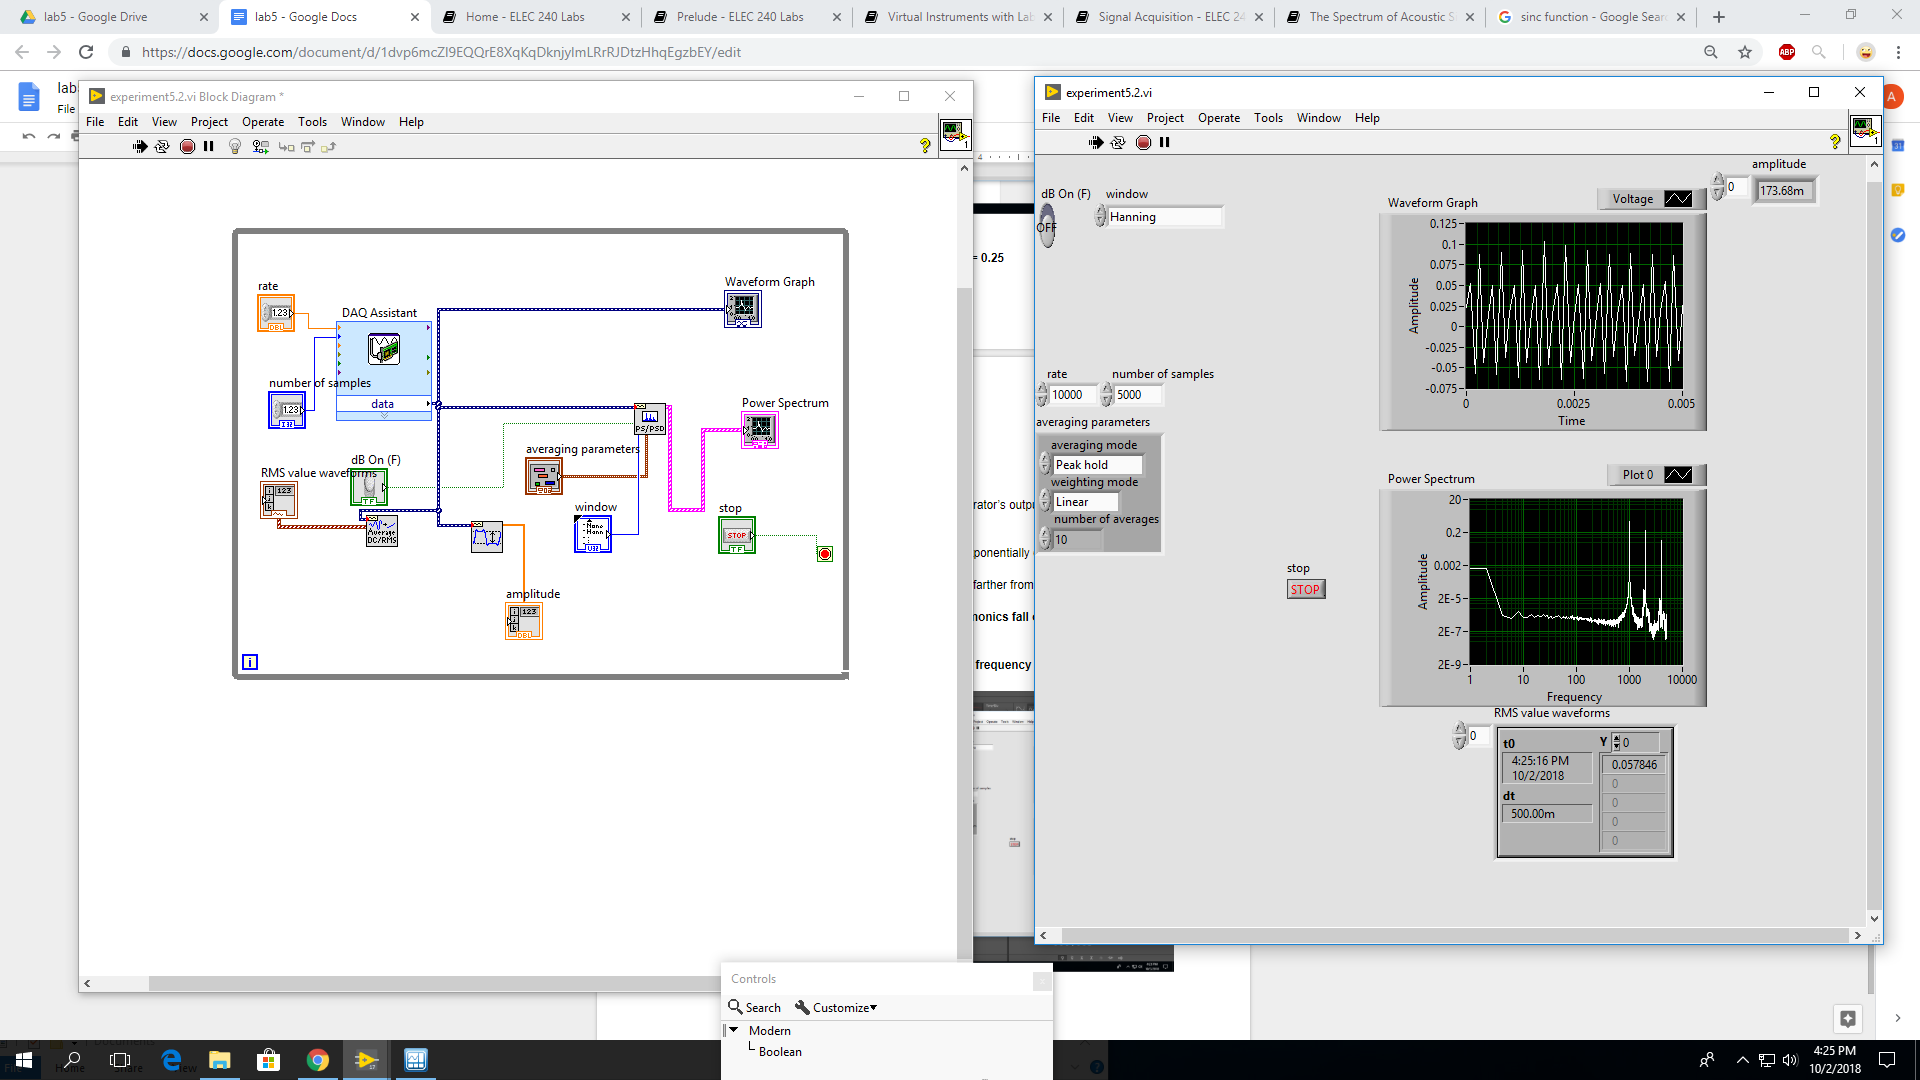
\includegraphics[scale=0.22]{images/124khztransferfunction.png}
		\caption{Frequency Response of RC Circuit at 1,2,and 4 kHz}
		\label{fig:124}
	\end{figure}
\end{centering}



\subsection{Experiment 5.3: The Spectrum of Acoustic Signals}

Using the circuit from last week, attach the spectrum analyzer across $V_out$. When trying to make a sustained a sound into the mic, the fundamental frequency was around 390 Hz. When changing sounds, it is clear that the frequency doesn't shift all that much, but the waveform changes. When keeping a constant "a" tone but changing pitch, the spectrum looks the same, but the lines change magnitude. Playing a whistle or a computer generated sound into the microphone leads to few harmonics and one large frequency. When comparing the output of the dynamic microphone and the telephone, it is clear that the dynamic microphone has less distortion. A fricative is a much sharper sound, with fewer lines on the spectrum and an avoiced fricative has even less, due to its sharp nature. After a series of tests, the bandwidth of sound seemed to be from 200 Hz to 1kHz, at a conservative estimate from Fig \ref{fig:mic}

\begin{centering}
	\begin{figure} [H]
		\centering
		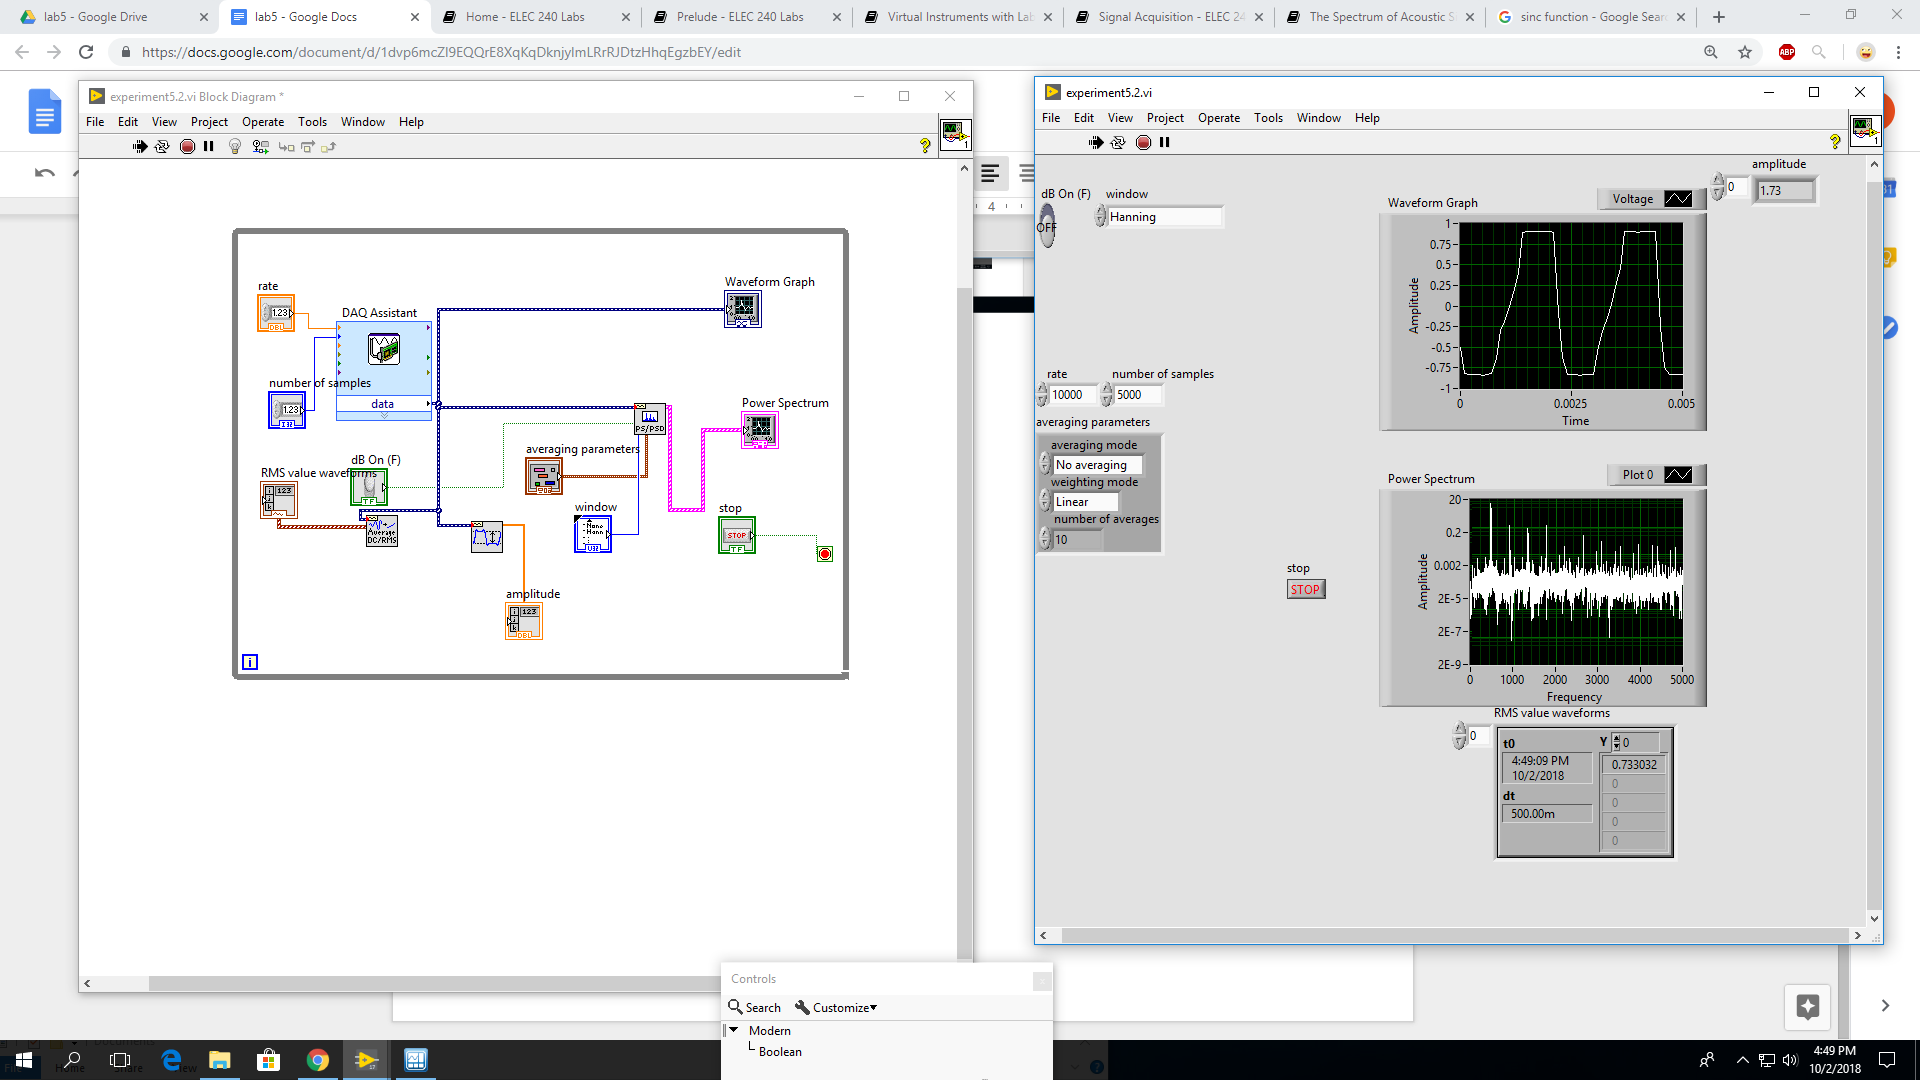
\includegraphics[scale=0.22]{images/mic.png}
		\caption{Power Spectrum of Speech Signal}
		\label{fig:mic}
	\end{figure}
\end{centering}


In Part B, we updated the circuit from last week once more, attaching the sound card in parallel with the dynamic microphone.  After running the Shepard tone through the spectrum analyzer, it was clear how it sounded like the pitch was always increasing. It consisted of three harmonics and the amplitude of the harmonics would cycle, leading it to sound like the pitch of the tone is constantly increasing. 


\section{References}

\begin{itemize}
	\item 	https://www.ece.rice.edu/~dpr2/elec240/lab5/
\end{itemize}

\medskip


\section{Conclusion}
In 5.1, we learned how to set up a circuit in LabView and learned about the various tools that LabView offers to aid in signal processing. For example, we learned that RMS averaging can help reduce the noisiness of the signal so that we can better observe its waveform. Furthemore, we learned that the peak-hold method was useful in finding the maximum power in a power spectrum graph. 

In 5.2, we learned how to acquire an external signal and process it inside of our LabView circuit. There are a variety of tools provided by LabView to assist in signal processing, including the RMS Voltage and amplitude measurer which allow us to measure these quantities. We also performed analysis on square and triangle waves by changing the duty cycle and the symmetry of the waves, respectively. We found that as we increased the duty cycle of the square wave, more spectral spikes occurred, which reflected the fact that more sine waves to construct a square wave with a duty cycle farther from 50\%. We noticed that as we decreased the symmetry of the triangle wave, the output waveform began to slant proportionally to the input triangle waveform's slant that we were modifying. 
We then proceeded to observe the spectrum of the signal with different axis settings. On a linear setting, we noticed that the spectrum appeared to fall off hyperbolically that represents how the harmonic frequencies exponentially decay in magnitude as frequency increases. By changing the y-axis to a log scale and setting a multiplier of 20, we were able to view a linear decrease in the spectrum as the harmonic frequency increased. 
In Part C, we measured the output of an RC circuit in LabView and passed a 1,2, and 4 kHz sine wave through the circuit. As expected, the magnitude of the output waveform fell by 6 db/Octave everytime we multipled the frequency by two because we were passing the signal through a low-pass filter, which attenuates higher frequencies more aggressively. 

In 5.3, we observed the spectrum of various speech signals. By observing the spectra of speech by both the dynamic microphone and the headset, we found that the dynamic microphone had less distortion. By observing figure 7, we estimate the approximate bandwidth of speech to occur from 200 Hz to 1 kHz. 
In Part B, we observed the spectrum of the Sheperd tone in real-time on the LabView display. It was then clear how the Sheperd tone worked; as a sine wave increased in frequency, it's magnitude would decrease, as seen by the decaying magnitude on the power spectrum as frequency increases. Thus, the signal achieves an effect of a perpetually increasing tone. 


\medskip


%\textit{Note (To be deleted): While the ``Results and Discussion'' section focused on the test results individually, the ``Conclusion'' discusses the results in the context of the entire experiment. Usually, the objectives given in the ``Introduction'' are reviewed to determine whether the experiment succeeded. If the objectives were not met, you should analyze why the results were not as predicted.}

\section{Errors}

%Your text here

\medskip
\begin{itemize}
	\item \textit{Handset microphone had excessive feedback:} Our handset, when placed facedown on a table or held in a certain position, would have excessive feedback, which would cause it to magnify the noise that it was producing. Thus, we would sometimes have to cover the earpiece so that we could speak into the microphone of the handset. However, this may not have perfectly insulated the earpiece from the microphone, so this likely exaggerated the distortion of the handset. In the future, use a higher quality/fully functional handset. 
\end{itemize}
%\textit{Note (To be deleted): Briefly list sources of error and discuss how to eliminate or deal with them}

\end{document}